\chapter{Architecture}
In this section we take a look at the relationships and organizational structure of the internal and external components that make up the \textit{myBank} banking application. The architecture description of our application defines several separate components and sub-components, each having clearly designed responsibilities. Interaction between components is controlled through the specification of interfaces. The goal of the design was to structure the application in such a way, that it would meet all requirements of the specification, while being well documented, maintainable and easily extensible in the future.
\section{Three Layer Structure}
Figure \ref{architecture} shows the main structure of the myBank application. The \textit{Smart-Card-Simulator} (\textit{SCS}) was not included in this figure, since it is regarded as an independent external component, which does not interact with the main myBank system. From a high abstraction level view, the application is structured into a classic three layers architecture. The fundamental layer at the bottom of the hierarchy is the \textit{Data Layer}. The main responsibility of this layer is to store and retrieve data. The \textit{Data Layer} offers an interface for data storage and retrieval functions, which is used by the \textit{Logic Layer}. This layer contains the ``meat'' of the banking application (\textit {business logic}), meaning that it contains the central components of the system, which are handling all logical tasks and are not part of the supporting infrastructure. This includes components responsible for Transactions, User management, Tan generation, Email dispatch and so on. The logic layer in turn offers functionality through an interface, that is used by the \textit{Presentation Layer} to display and manipulate information on the user level. In general we made sure, that components of each layer are only allowed to use the next lower layer through a specified interface, although our application does not strictly adhere to this in all cases.
%++++++++++++++++++++++++++++++++++++++++++++++++++++++
%+    Figure 1: myBank Component Overview             +
%++++++++++++++++++++++++++++++++++++++++++++++++++++++
\begin{center}
\begin{figure}[hbtp]
        \centering
        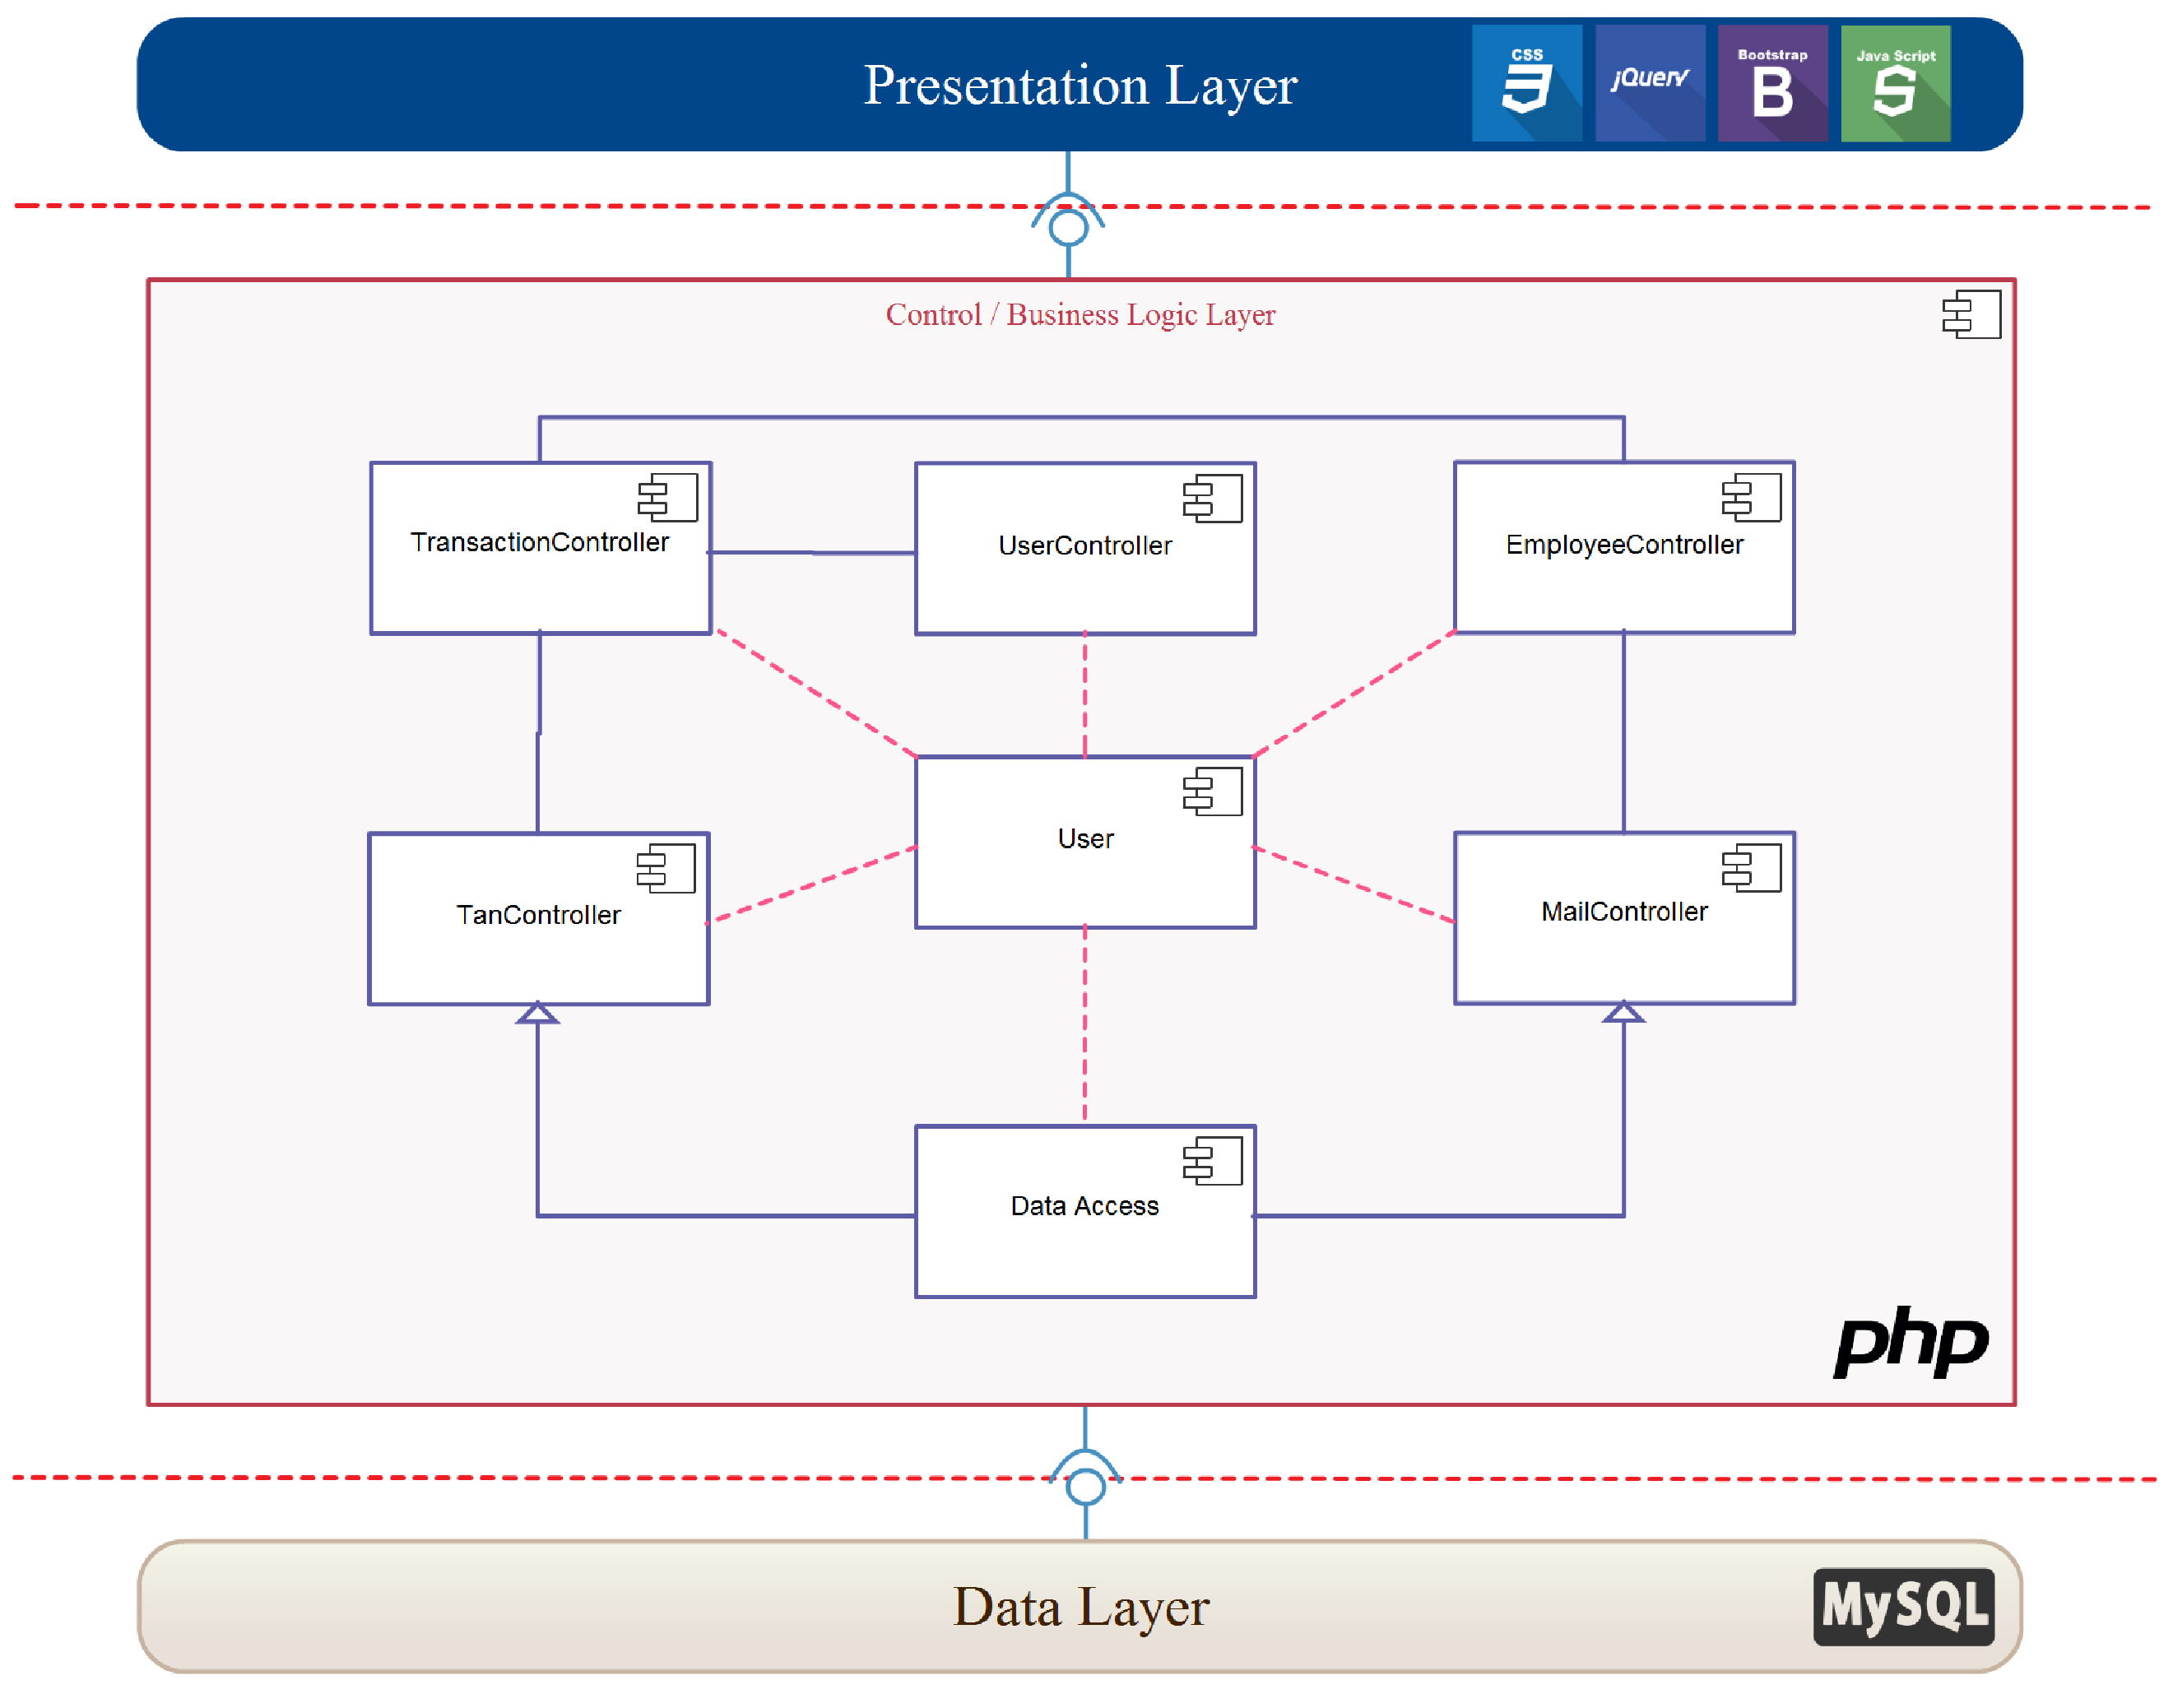
\includegraphics[width=1.0\linewidth]{architecture}
        \caption{myBank Component Overview}\label{architecture}
\end{figure}
\end{center}
\section{Logic Layer Components: Separation of Concerns}
The sub-components of the logic layer clearly encapsulate related functionality and are designed to function as independently as possible. Moreover, components and modules are clearly named according to their responsibilities. This makes a complex system easier to understand and limits the possibility for confusion, due to inappropriately named modules. The important components of the logic layer are:
\begin{itemize}

  \item Data Access
  \item User
  \item User Controller
  \item Tan Controller
  \item Transaction Controller
  \item Employee Controller
  \item Mail Controller

\end{itemize}
The flow of data is generally designed to be from bottom to top, as indicated by the arrows in figure \ref{architecture}. Dependencies between components are designed to be minimal. Most components depend on a maximum of one or two other components, which also limits their communication channels, improving maintainability and ease of use. The following list gives some insight into the functionality that is encapsulated by each of the main logic layer components. We would like to note, that we realize, the architecture is not perfect and there is still room for improving the independence of components and their modules.
\begin{description}
  \item[Data Access] \hfill \\
  Abstracts access to the data layer. Main task is insertion and retrieval of data through communication with the mysql database.
  \item[User] \hfill \\
  Abstracts a user or employee of the System. The myBank application is a user centric system, meaning that the user (customer or employee) is the central component of the system and is involved in almost all operations performed at the logic layer. Since the User class is used by nearly all sub-components, it is designed to be very concise and lightweight.
  \item[User Controller] \hfill \\
  Offers functionality to verify user and employee credentials, as well as control over the lockout mechanisms.
  \item[Tan Controller] \hfill \\
  Responsible for generation, verification, selection and maintenance of transaction numbers.
  \item[Transaction Controller] \hfill \\
  Implements functionality for credit transfers between users. Each transaction involves a large number of steps, including the validity of transaction data, verification of credentials, checking of available funds, selection of TANs and so on. These steps are abstracted into an easy to use interface by the Transaction Controller.
  \item[Employee Controller] \hfill \\
  Offers employee functionality, such as approval of users and transactions over the limit of 10000 Credits.
  \item[Mail Controller] \hfill \\
  As the name suggests, this component is tasked with sending out Emails to customers.
\end{description}
Figure \ref{hierarchy} shows a more granular view of some system modules on the function level. The figure shows a functional hierarchy for parts of the Mail Controller, User Controller and Data Access. In the body of each function dependencies are listed, some of which are external and not included in this view to abstract from the complexity.
%++++++++++++++++++++++++++++++++++++++++++++++++++++++
%+    Figure 2: myBank Functional Hierarchy           +
%++++++++++++++++++++++++++++++++++++++++++++++++++++++
\begin{center}
\begin{figure}[hbtp]
        \centering
        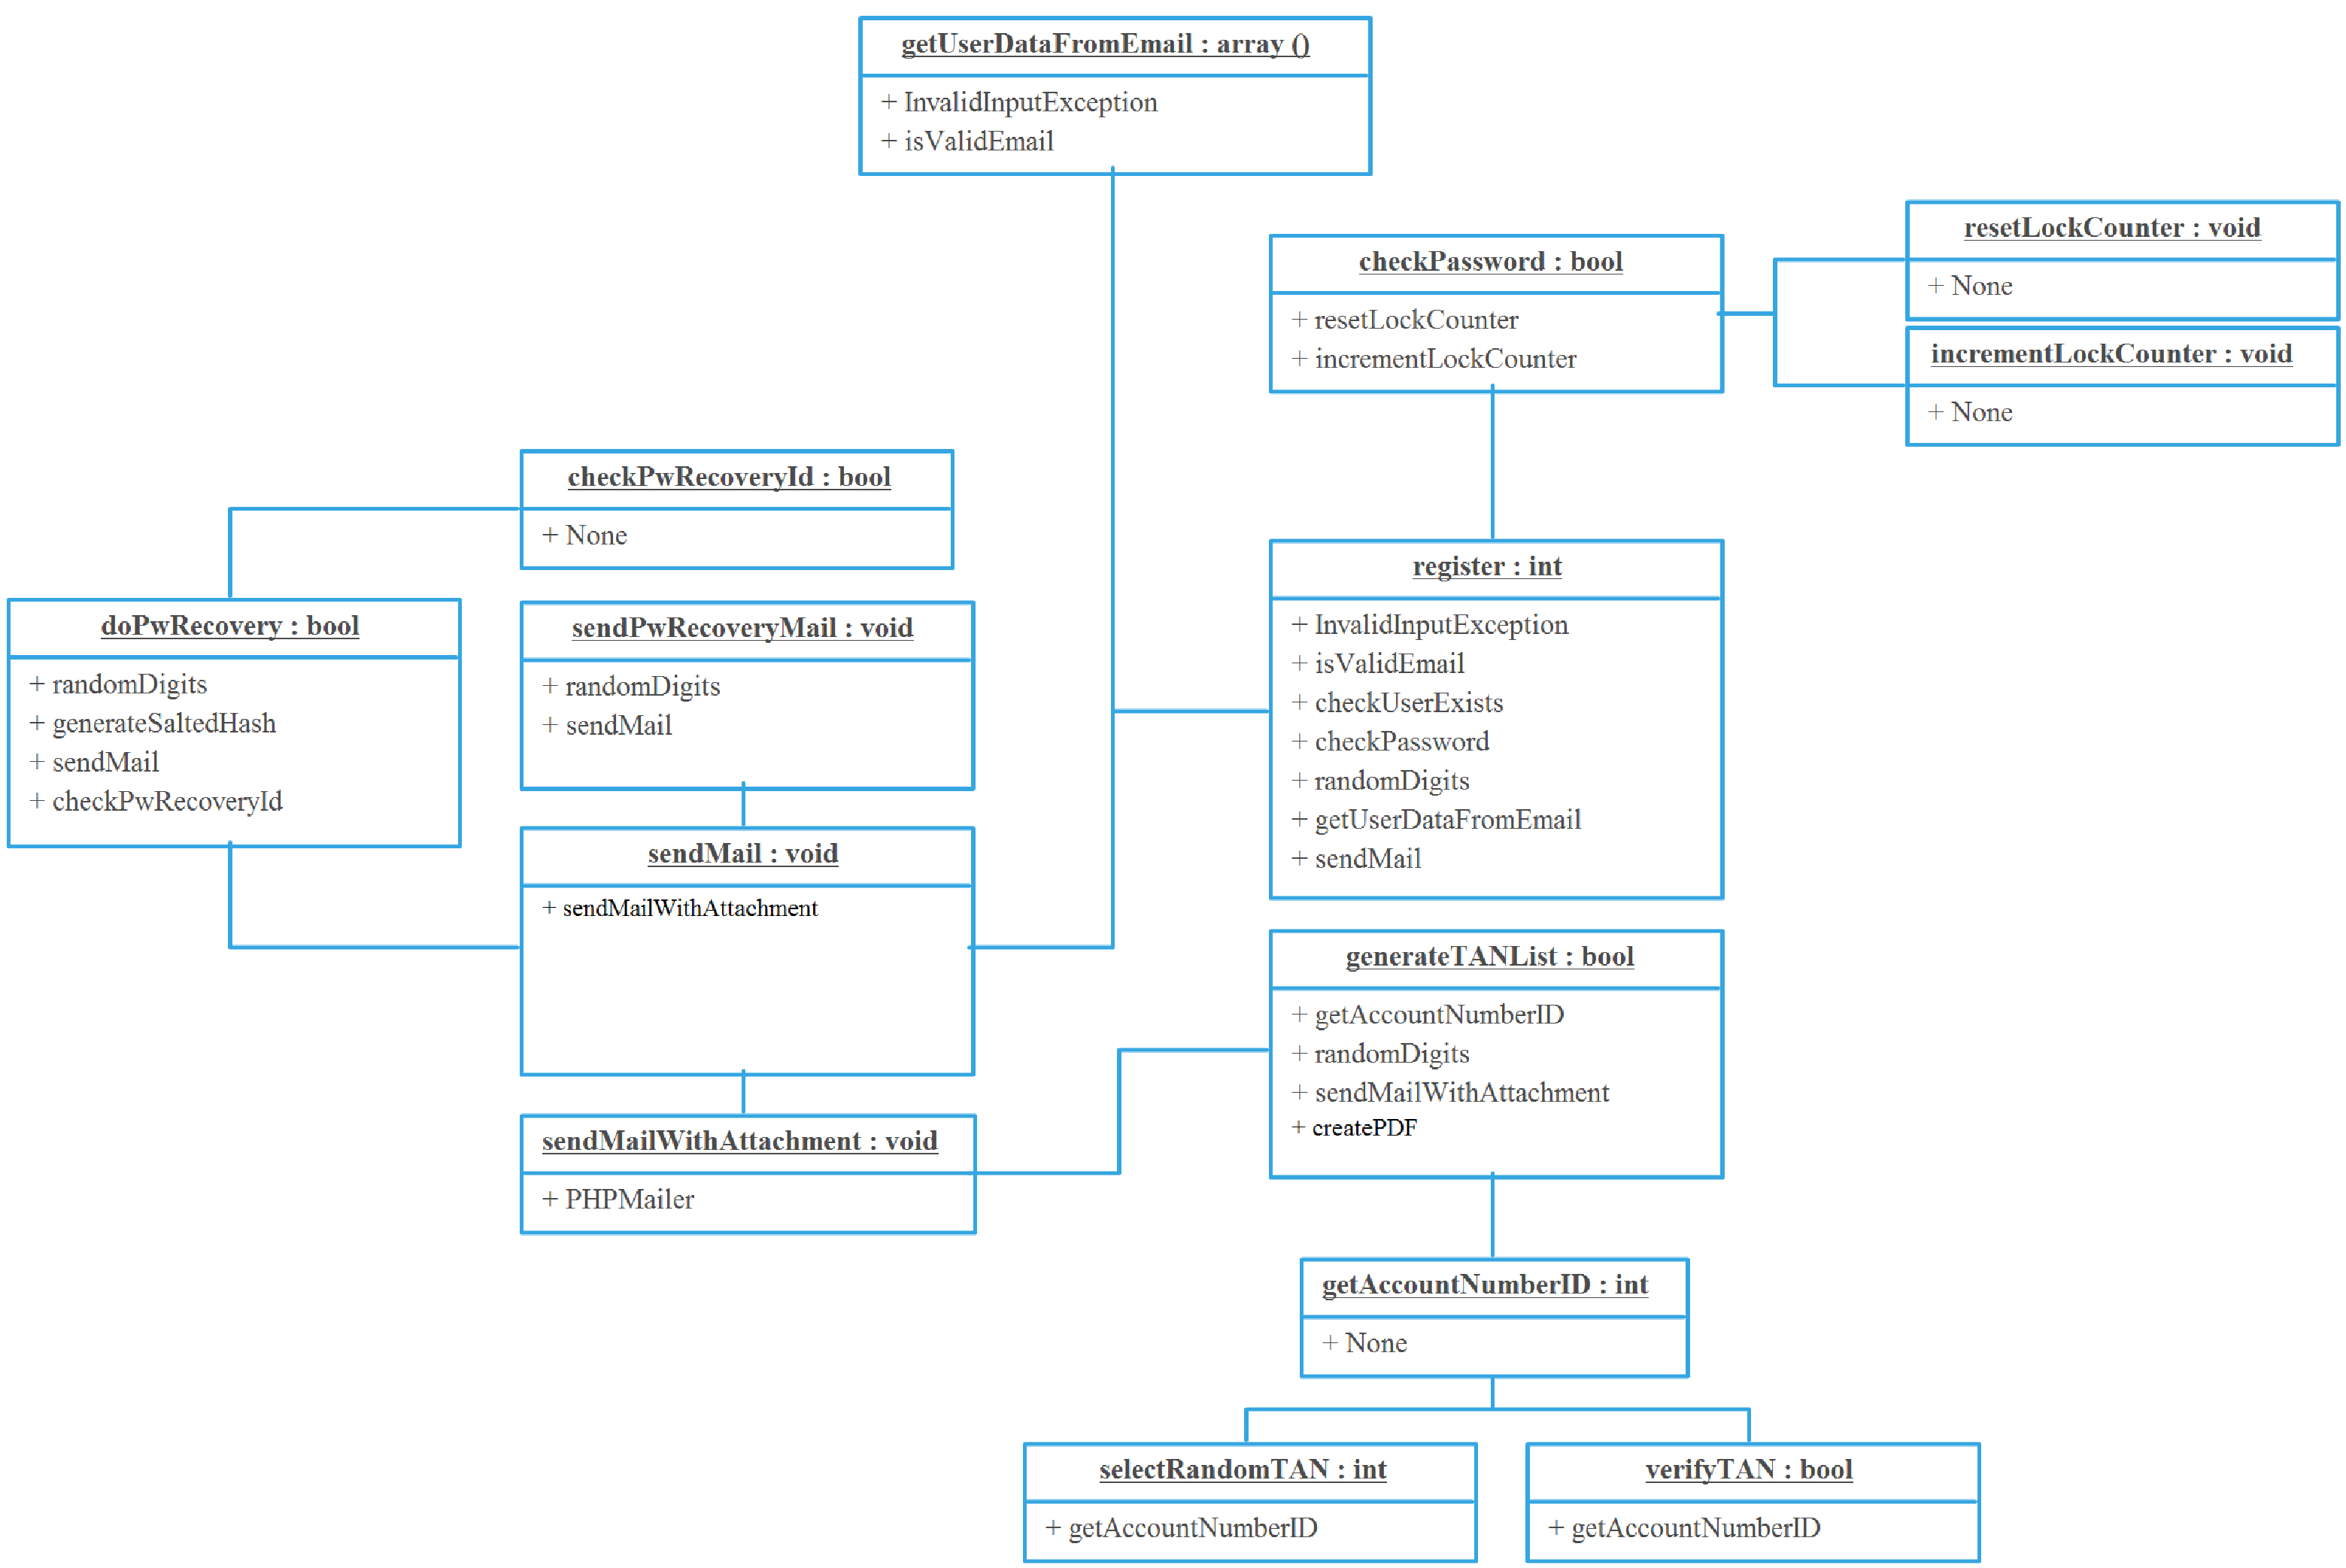
\includegraphics[width=1.0\linewidth]{hierarchy}
        \caption{myBank Function Hierarchy Excerpt}\label{hierarchy}
\end{figure}
\end{center}
\section{Technologies \& Languages}
The myBank application makes use of several different technologies on each layer. The following is a list of technologies and programming/scripting languages utilized by layer.
\begin{description}
  \item[Presentation Layer] \hfill \\
  HTML5, CSS3, JavaScript, Twitter Bootstrap (front-end framework), Yahoo! pure
  \item[Logic Layer] \hfill \\
  PHP 5.3/4, Java, C
  \item[Data Layer] \hfill \\
  MySQL
\end{description}